\documentclass{article}
\usepackage[utf8]{inputenc}
\usepackage{amsmath} % Advanced math typesetting
\usepackage[utf8]{inputenc} % Unicode support (Umlauts etc.)
\usepackage[ngerman]{babel} % Change hyphenation rules
\usepackage{hyperref} % Add a link to your document
\usepackage[final]{graphicx} % Add pictures to your document
\usepackage{listings} % Source code formatting and highlighting
\usepackage{bookmark}
\usepackage{natbib}
\usepackage{geometry}
\usepackage{multicol}
\usepackage{fancyhdr}
\usepackage[document]{ragged2e}
 
\pagestyle{fancy}
\fancyhf{}
\fancyhead[LE,RO]{Overleaf}
\fancyhead[RE,LO]{Guides and tutorials}
\fancyfoot[CE,CO]{\leftmark}
\fancyfoot[LE,RO]{\thepage}
\graphicspath{{Immagini//}}
%C:\Users\erikz\OneDrive\Desktop\PaioPaio2\IMM-Sensors-Network\Latex\Immagini
\geometry{
 a4paper,
 total={170mm,257mm},
 left=20mm,
 top=20mm,
 }

\title{Imm algorithm implementation for tracking}
\author{
Paiola Lorenzo 000000 

Zanolli Erik 198852}
\date{January 2020}





\begin{document}

\maketitle



\section*{Introduction}
\justify
The porpouse of this document is the analysis and performance evaluation of an IMM algorithm's implementation in
a sensor grid tracking an object. The object can move with two different model, random walk and unicycle, governed by
 a Markov chain. The goal is evaluate the best trade-off between error on estimated position and real position and number of 
 messagesses involved in tracking

\begin{multicols}{2}
    \section*{Backgound}
    \justify
        Tracking a object with a changing dynamic require propers algorithms and filters. Retriving physical data with
        observations it's not enough, models achiving the best-fit to our data is needed in order to make a prediction and estimate 
        with reduced uncertainty. Here comes to play a major role the IMM algorithm (Interacting Multiple Models): The data
        from sensor are combined with different dynamical models through the algorithm... 
        \subsection*{Sensor in simulation model}
            The target can move with random movement described by a Markov chain and accordingly two different models of movement
            The tracking are performed with grid of sensors. In order to perform a proper simulation the sensor has assumed to have a limited
            range for the tracking and we cannot retrive any information if target is out. It also took in consideration the power consumption 
            for a possible physical system: to model a more enegy efficient system the sensor can switch to 3 different working condition: On,Off,Idle.
            To achive this goal the sensor is working as a state machine as showned in the figure below: 
                \begin{figure}[h!]
                \centering
                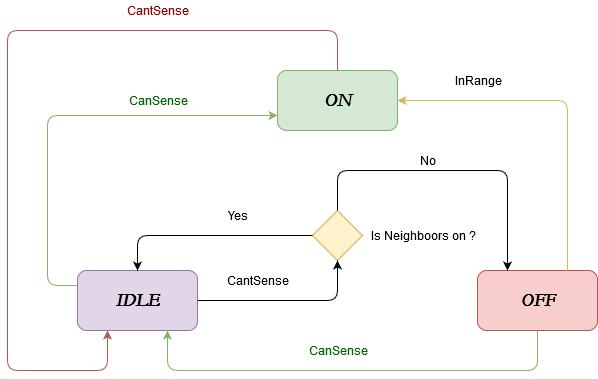
\includegraphics[scale=0.05]{UntitledDiagram.png}
                \caption{State machine sensor}
                \label{fig:galaxy}
                \end{figure}
            Sensors can communicate with the sensors in their neighboorhoods and exchange signal named CanSense and CantSense that regulate the transition
            between differents state. Thus implies that not all the sensors receive all the messagge, but only from their Neighboors. The sensors in On state
            create a fully connected graph. The nodes composing the graph changes dynamically with iterations according with the movements of target. The numbers of
            sensors turned on depends on working range choosed and position of target. The mechanism that regulate the transition from sensors state 
            relay on the information exchanged with nearby sensor. Different state can receive and send different messagesses. A sensor in On state has the moving 
            object in his range and send a CanSense to the nearby and when trackin moving away from the operating range send a CantSense turning itself to Idle. 
            Sensors that receive a CanSense and are not already On turn in Idle state; during the Idle state sensors check
            if object appears in range sensors turn to On and send a CanSense, if nothing trigger the range it send to the nearby a CantSense signal.
            A sensor that is in Idle and during the information exchange receive only CantSense from the nearby turn itself Off and stop to check if somenthing is in range and
            can be turned again to Idle via a CanSense. This scheme implies that a sensors can never switch to On from Off except for the initialization step. 
            When a sensor have the target in range it does a measure operation each timestep. the sensor works a radar in this model and remembering
            \begin{equation}
                z(k)=H(k)x(k)+\textbf{R}
            \end{equation}
            where the \textbf{H} is 
            \begin{equation}
                H= \begin{bmatrix}
                    dopo & la \\
                    scr & vo \\
                \end{bmatrix}
            \end{equation} 
        \subsection*{Imm and Linear Consensu}
               The IMM algorithm is based on the 
                
    \section*{Model used}
    Introduction
    
    \subsection*{Random walk and Unycicle model}
    The target in this simulation can move accordingly to two model: random walk and Unycicle. Each of this model has a Markov chain that 
    regulate how the given input goes in the system. For the random walk we have 5 state: costant velocity, positive or negative acceleration
     on x direction and positive or negative deceleration on y direction. So the input are $\ddot{x}$ and $\ddot{y}$. The Markov chain associate is a circulant matrix as showned below
     $$\begin{vmatrix}
         0.8 & 0.025 & 0.025 & 0.025 & 0.025 // 
     \end{vmatrix}$$
     The equation regulating the state of the system is as well know
    \begin{equation}
    X^{+}= \textbf{A}X(k) + \textbf{B}u(k) + \textbf{G}w(k)
    \end{equation}
    The Random walk model has is a linear model. State,state and noise matrix associate to the random walk has showned below:
    \[ X=\begin{bmatrix} x \\ y \\ \dot{x} \\ \dot{y} \\ \end{bmatrix}  A=\begin{bmatrix}
        1&0&\delta&0\\
        0&1&0&\delta\\
        0&0&1&0\\
        0&0&0&1\\
        \end{bmatrix}
        G=\begin{bmatrix}
            \delta^2/2&0\\
            0&\delta^2/2\\
            \delta&0\\
            0&\delta\\
            \end{bmatrix}
        \]
        The \textbf{B} input matrix change accordingly with the acceleration input
    \[
        B=\begin{bmatrix}
            \delta^2/2 & 0\\
            0 & 0  \\
            \delta & 0 \\
            0 & 0 \\
            \end{bmatrix}
            B=\begin{bmatrix}
                0 & 0 \\
             0 & \delta^2/2 \\
            0 & 0 \\
            0 & \delta \\
            \end{bmatrix}
  \]
  It can be noticed that the \textbf{G} matrix of error can be seen as a sum of positive \textbf{B} rescaled by a random factor.

  The unycicle model has different input and state description. The inputare represente by the angular acceleration of the wheel and the steering angle acceleration.
  possible state are 5: constant angular velocity, acceleration and deceleration of the wheel and positice or negative acceleration of the steering angle.
  The associate Markov chain for this case is  
   $$\begin{vmatrix}
         0.8 & 0.025 & 0.025 & 0.025 & 0.025 // 
     \end{vmatrix}$$
   Unycicle model instead is a Non-linear model. Thus is necessary to use a linearization in the Kalman filter implementation
   The matrix that represent the state of system for this case are
    \[ X=\begin{bmatrix} x \\ y \\ \dot{x} \\ \dot{y} \\ \end{bmatrix}  A=\begin{bmatrix}
   1&0&\delta&0\\
   0&1&0&\delta\\
   0&0&1&0\\
   0&0&0&1\\
   \end{bmatrix}
   G=\begin{bmatrix}
       \delta^2/2&0\\
       0&\delta^2/2\\
       \delta&0\\
       0&\delta\\
       \end{bmatrix}
   \]
    \subsection*{Data's simulation}

    \section*{Result}
    The performance evaluation of the system are evaluted by computing the RMS of the predicted trajectory eith the respect to the actual one 
    choosing different rate of performind the WSL. The final result are listed in the table below
    

\begin{center}
    \begin{tabular}{||c c c c||} 
    \hline
    1 step & 2 step & 3 step & 4 step \\ [0.5ex] 
    \hline\hline
    1 & 6 & 87837 & 787 \\ 
    \hline
    2 & 7 & 78 & 5415 \\
    \hline
    3 & 545 & 778 & 7507 \\
    \hline
    4 & 545 & 18744 & 7560 \\
    \hline
    5 & 88 & 788 & 6344 \\ [1ex] 
    \hline
   \end{tabular}
   \end{center}
   
   
    \subsection*{}
\end{multicols}
\end{document}
